\subsubsection{UC16 - Gestione Fatture}
\begin{figure}[h]
	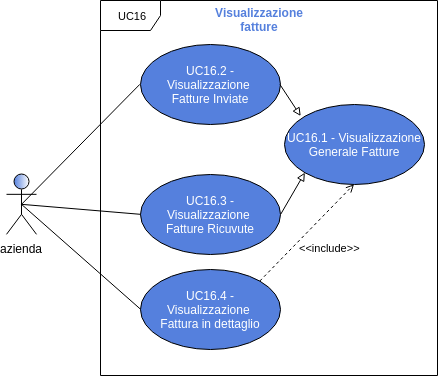
\includegraphics[width=8cm]{res/images/UC16-Generale.png}
	\centering
	\caption{UC14.3 -Visualizzazione delle fatture}
\end{figure}
\begin{itemize}
	\item \textbf{Attori Primari}: azienda;
	\item \textbf{Descrizione}: l'azienda può visualizzare tutte le fatture emesse e ricevute;
	\item \textbf{Scenario principale}: l'utente visualizza le liste di tutte le fatture emesse e ricevute;
	\item \textbf{Precondizione}: il sistema ha riconosciuto l'utente autenticato come azienda, l'utente ha espresso la volontà di visualizzare una delle liste di fatture;
	\item \textbf{Postcondizione}: l'azienda ha visualizzato le proprie fatture.
\end{itemize}
\subsubsection{UC16.1 - Visualizzazione Generale Fatture}
\begin{figure}[h]
	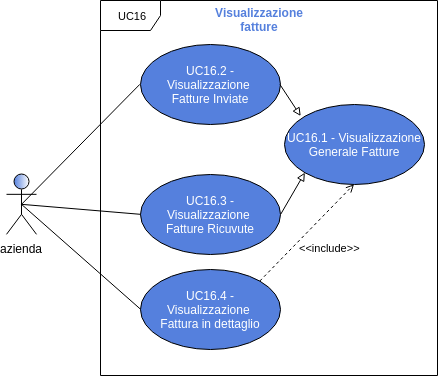
\includegraphics[width=8cm]{res/images/UC16-Generale.png}
	\centering
	\caption{UC14.3 - Dettagli campi visualizzati per una fattura in una lista}
\end{figure}
\begin{itemize}
	\item \textbf{Attori Primari}: azienda;
	\item \textbf{Descrizione}: per ogni fattura presente in una lista di fatture, l'utente visualizza la data, il numero identificativo e l'importo totale; 
	\item \textbf{Scenario principale}: l'utente visualizza le fatture riguardanti gli acquisti o le vendite;
	\item \textbf{Specializzazioni}:
	\begin{itemize}
		\item \textbf{UC16.2}: visualizzazione delle fatture inviate; 
		\item \textbf{UC16.3}: visualizzazione delle fatture ricevute;
	\end{itemize}
	\item \textbf{Precondizione}: il sistema ha riconosciuto l'utente autenticato come azienda, l'utente ha espresso la volontà di visualizzare le fatture;
	\item \textbf{Postcondizione}: l'azienda ha visualizzato le proprie fatture, in cui sono presenti la data, in numero identificativo e l'importo totale.
\end{itemize} 
\subsubsection{UC16.1.1 - Visualizzazione Data Fattura}
\begin{itemize}
	\item \textbf{Attori Primari}: azienda;
	\item \textbf{Descrizione}: l'azienda visualizza la data della fattura;
	\item \textbf{Scenario principale}: l'utente visualizza una lista delle fatture, per ogni fattura visualizza la relativa data;
	\item \textbf{Precondizione}: il sistema ha riconosciuto l'utente autenticato come azienda, l'utente ha espresso la volontà di visualizzare una delle liste di fatture;
	\item \textbf{Postcondizione}: l'azienda ha visualizzato le proprie fatture, in particolare ha visualizzato le relative date.
\end{itemize} 
\subsubsection{UC16.1.2 - Visualizzazione Numero fattura}
\begin{itemize}
	\item \textbf{Attori Primari}: azienda;
	\item \textbf{Descrizione}: l'azienda visualizza il numero identificativo della fattura;
	\item \textbf{Scenario principale}: l'utente visualizza una lista delle fatture, per ogni fattura visualizza il numero identificativo della fattura;
	\item \textbf{Precondizione}: il sistema ha riconosciuto l'utente autenticato come azienda, l'utente ha espresso la volontà di visualizzare una delle liste di fatture;
	\item \textbf{Postcondizione}: l'azienda ha visualizzato le proprie fatture, in particolare ha visualizzato il numero identificativo delle fatture.
\end{itemize} 

\subsubsection{UC16.1.3 - Visualizzazione Importo totale}
\begin{itemize}
	\item \textbf{Attori Primari}: azienda;
	\item \textbf{Descrizione}: l'azienda visualizza l'importo totale della fattura;
	\item \textbf{Scenario principale}: l'utente visualizza una lista delle fatture, per ogni fattura visualizza il relativo importo totale;
	\item \textbf{Precondizione}: il sistema ha riconosciuto l'utente autenticato come azienda, l'utente ha espresso la volontà di visualizzare una delle liste di fatture;
	\item \textbf{Postcondizione}: l'azienda ha visualizzato le proprie fatture, in particolare ha visualizzato i relativi importi totali.
\end{itemize} 

\subsubsection{UC16.2 - Visualizzazione Fatture Inviate}
\begin{figure}[h]
	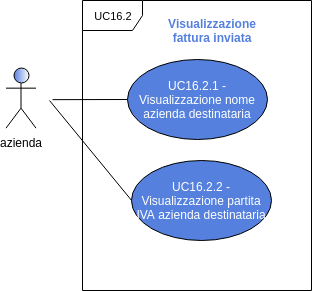
\includegraphics[width=6cm]{res/images/UC16-VisualizzazioneFatturaInviata.png}
	\centering
	\caption{UC16.2 - Campi aggiuntivi nella visualizzazione di una fattura inviata}
\end{figure}
\begin{itemize}
	\item \textbf{Attori Primari}: azienda;
	\item \textbf{Descrizione}: l'azienda visualizza le fatture inviate ad altre aziende;
	\item \textbf{Scenario principale}: l'utente visualizza una lista contenente le fatture inviate alle aziende-clienti, ed oltre ai dati generali sono presenti anche il nome e la partita IVA dell'azienda-cliente;
	\item \textbf{Precondizione}: il sistema ha riconosciuto l'utente autenticato come azienda, l'utente ha espresso la volontà di visualizzare le fatture inviate ad altre aziende;
	\item \textbf{Postcondizione}: l'azienda ha visualizzato la lista contenente tali fatture, potendo leggere il nome e la partita IVA delle aziende-clienti.
\end{itemize}
\subsubsection{UC16.2.1 - Visualizzazione nome azienda destinataria}
\begin{itemize}
	\item \textbf{Attori Primari}: azienda;
	\item \textbf{Descrizione}: l'azienda visualizza il nome dell'azienda destinataria della fattura;
	\item \textbf{Scenario principale}: l'utente visualizza la lista delle fatture inviate, per ogni fattura visualizza il relativo nome dell'azienda destinataria;
	\item \textbf{Precondizione}: il sistema ha riconosciuto l'utente autenticato come azienda, l'utente ha espresso la volontà di visualizzare la lista delle fatture inviate;
	\item \textbf{Postcondizione}: l'azienda ha visualizzato la lista delle proprie fatture inviate, in particolare ha visualizzato i relativi nomi delle aziende destinatarie.
\end{itemize} 
\subsubsection{UC16.2.2 - Visualizzazione partita IVA azienda destinataria}
\begin{itemize}
	\item \textbf{Attori Primari}: azienda;
	\item \textbf{Descrizione}: l'azienda visualizza la partita IVA dell'azienda destinataria della fattura;
	\item \textbf{Scenario principale}: l'utente visualizza la lista delle fatture inviate, per ogni fattura visualizza la relativa partita IVA dell'azienda destinataria;
	\item \textbf{Precondizione}: il sistema ha riconosciuto l'utente autenticato come azienda, l'utente ha espresso la volontà di visualizzare la lista delle fatture inviate;
	\item \textbf{Postcondizione}: l'azienda ha visualizzato la lista delle proprie fatture inviate, in particolare ha visualizzato le partite IVA delle aziende destinatarie.
\end{itemize} 



\subsubsection{UC16.3 - Visualizzazione Fatture Ricevute}
\begin{figure}[h]
	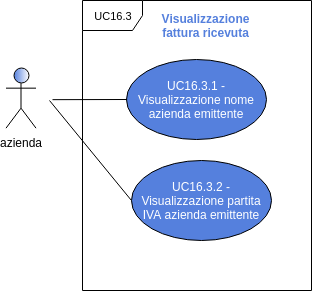
\includegraphics[width=6cm]{res/images/UC16-VisualizzazioneFatturaRicevuta.png}
	\centering
	\caption{UC16.3 - Campi aggiuntivi nella visualizzazione di una fattura ricevuta}
\end{figure}

\begin{itemize}
	\item \textbf{Attori Primari}: azienda;
	\item \textbf{Descrizione}: l'azienda visualizza le fatture ricevute dalle altre aziende;
	\item \textbf{Scenario principale}: l'utente visualizza una lista contenente le fatture ricevute dalle aziende-venditrici, ed oltre ai dati generali sono presenti anche il nome e la partita IVA dell'azienda emittente;
	\item \textbf{Precondizione}: il sistema ha riconosciuto l'utente autenticato come azienda, l'utente ha espresso la volontà di visualizzare le fatture ricevute da altre aziende;
	\item \textbf{Postcondizione}: l'azienda ha visualizzato la lista contenente tali fatture, potendo leggere il nome e la partita IVA delle aziende-venditrici.
\end{itemize}
\subsubsection{UC16.3.1 - Visualizzazione nome azienda destinataria}
\begin{itemize}
	\item \textbf{Attori Primari}: azienda;
	\item \textbf{Descrizione}: l'azienda visualizza il nome dell'azienda emittente nella fattura;
	\item \textbf{Scenario principale}: l'utente visualizza la lista delle fatture ricevute, per ogni fattura visualizza il relativo nome dell'azienda emittente;
	\item \textbf{Precondizione}: il sistema ha riconosciuto l'utente autenticato come azienda, l'utente ha espresso la volontà di visualizzare la lista delle fatture ricevute;
	\item \textbf{Postcondizione}: l'azienda ha visualizzato la lista delle proprie fatture ricevute, in particolare ha visualizzato i relativi nomi delle aziende emittenti.
\end{itemize} 
\subsubsection{UC16.3.2 - Visualizzazione partita IVA azienda destinataria}
\begin{itemize}
	\item \textbf{Attori Primari}: azienda;
	\item \textbf{Descrizione}: l'azienda visualizza la partita IVA dell'azienda emittente nella fattura;
	\item \textbf{Scenario principale}: l'utente visualizza la lista delle fatture ricevute, per ogni fattura visualizza la relativa partita IVA dell'azienda emittente;
	\item \textbf{Precondizione}: il sistema ha riconosciuto l'utente autenticato come azienda, l'utente ha espresso la volontà di visualizzare la lista delle fatture ricevute;
	\item \textbf{Postcondizione}: l'azienda ha visualizzato la lista delle proprie fatture ricevute, in particolare ha visualizzato le relative partite IVA delle aziende emittenti.
\end{itemize}  


\subsubsection{UC16.4 - Visualizzazione Fattura in dettaglio}
\begin{figure}[h]
	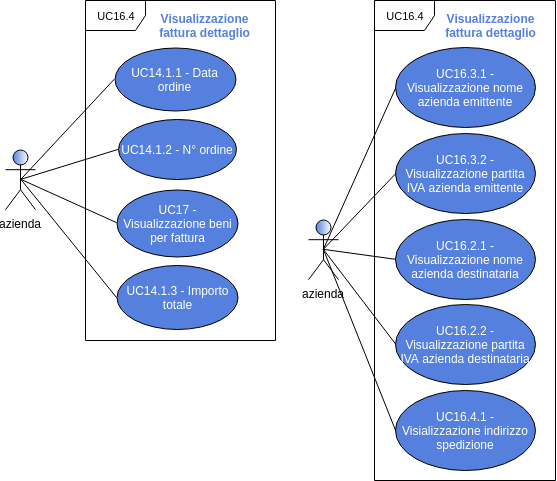
\includegraphics[width=10cm]{res/images/UC16-VisualizzazioneFatturaDettaglio.png}
	\centering
	\caption{UC16.3 - Campi della visualizzazione dettagliata di una fattura}
\end{figure}
\begin{itemize}
	\item \textbf{Attori Primari}: azienda;
	\item \textbf{Descrizione}: l'azienda può leggere tutti i dettagli di una fattura;
	\item \textbf{Scenario principale}: l'azienda seleziona una fattura da una lista e può leggere tutti i dettagli di tale fattura. Essi sono:
		\begin{enumerate}[label=\alph*.]
		\item la data dell'ordine relativo alla fattura [UC14.1.1];
		\item il numero identificativo dell'ordine relativo alla fattura [14.1.2];
		\item visualizzazione dei beni in formato fattura [UC17];
		\item l'importo totale dell'ordine [UC14.1.3];
		\item il nome dell'azienda emittente [UC16.3.1];
		\item la partita IVA dell'azienda emittente [UC16.3.2];
		\item il nome dell'azienda destinataria [UC16.2.1];
		\item la partita IVA dell'azienda destinataria [UC16.2.2];
		\item indirizzo di spedizione dell'ordine [UC16.4.1];
	\end{enumerate}
	\item \textbf{Inclusioni}:
	\begin{itemize}
		\item \textbf{UC16.3}: per poter accedere ai dettagli di una particolare fattura è necessario selezionarla da una delle liste disponibili;
	\end{itemize}
	\item \textbf{Precondizione}: il sistema ha riconosciuto l'utente autenticato come azienda, l'utente ha espresso la volontà di visualizzare i dettagli di una specifica fattura;
	\item \textbf{Postcondizione}: l'azienda ha visualizzato i dettagli della fattura selezionata. In particolare 
\end{itemize} 
\subsubsection{UC16.4.1 - Visualizzazione indirizzo di spedizione dell'ordine}
\begin{itemize}
	\item \textbf{Attori Primari}: azienda;
	\item \textbf{Descrizione}: l'azienda visualizza l'indirizzo di spedizione relativo all'ordine nella fattura;
	\item \textbf{Scenario principale}: l'utente visualizza una fattura in dettaglio. Tra i dati è presente l'indirizzo di spedizione dell'ordine a cui si riferisce la fattura;
	\item \textbf{Precondizione}: il sistema ha riconosciuto l'utente autenticato come azienda, l'utente ha espresso la volontà di visualizzare una fattura in dettaglio;
	\item \textbf{Postcondizione}: l'azienda ha visualizzato tale fattura in dettaglio, in particolare ha visualizzato l'indirizzo di spedizione dell'ordine.
\end{itemize} 
